\documentclass{tufte-book}

\hypersetup{colorlinks}% uncomment this line if you prefer colored hyperlinks (e.g., for onscreen viewing)

%%
% Book metadata
\title{A Tufte-Style Book\thanks{Thanks to Edward R.~Tufte for his inspiration.}}
\author[The Tufte-LaTeX Developers]{The Tufte-LaTeX\ Developers}
\publisher{Publisher of This Book}

%%
% If they're installed, use Bergamo and Chantilly from www.fontsite.com.
% They're clones of Bembo and Gill Sans, respectively.
%\IfFileExists{bergamo.sty}{\usepackage[osf]{bergamo}}{}% Bembo
%\IfFileExists{chantill.sty}{\usepackage{chantill}}{}% Gill Sans

%\usepackage{microtype}

%%
% Just some sample text
\usepackage{lipsum}

%%
% For nicely typeset tabular material
\usepackage{booktabs}

%%
% For graphics / images
\usepackage{graphicx}
\setkeys{Gin}{width=\linewidth,totalheight=\textheight,keepaspectratio}
\graphicspath{{graphics/}}

% The fancyvrb package lets us customize the formatting of verbatim
% environments.  We use a slightly smaller font.
\usepackage{fancyvrb}
\fvset{fontsize=\normalsize}

%%
% Prints argument within hanging parentheses (i.e., parentheses that take
% up no horizontal space).  Useful in tabular environments.
\newcommand{\hangp}[1]{\makebox[0pt][r]{(}#1\makebox[0pt][l]{)}}

%%
% Prints an asterisk that takes up no horizontal space.
% Useful in tabular environments.
\newcommand{\hangstar}{\makebox[0pt][l]{*}}

%%
% Prints a trailing space in a smart way.
\usepackage{xspace}

\usepackage{pbox}
%%
% Some shortcuts for Tufte's book titles.  The lowercase commands will
% produce the initials of the book title in italics.  The all-caps commands
% will print out the full title of the book in italics.
\newcommand{\vdqi}{\textit{VDQI}\xspace}
\newcommand{\ei}{\textit{EI}\xspace}
\newcommand{\ve}{\textit{VE}\xspace}
\newcommand{\be}{\textit{BE}\xspace}
\newcommand{\VDQI}{\textit{The Visual Display of Quantitative Information}\xspace}
\newcommand{\EI}{\textit{Envisioning Information}\xspace}
\newcommand{\VE}{\textit{Visual Explanations}\xspace}
\newcommand{\BE}{\textit{Beautiful Evidence}\xspace}

\newcommand{\TL}{Tufte-\LaTeX\xspace}

% Prints the month name (e.g., January) and the year (e.g., 2008)
\newcommand{\monthyear}{%
  \ifcase\month\or January\or February\or March\or April\or May\or June\or
  July\or August\or September\or October\or November\or
  December\fi\space\number\year
}


% Prints an epigraph and speaker in sans serif, all-caps type.
\newcommand{\openepigraph}[2]{%
  %\sffamily\fontsize{14}{16}\selectfont
  \begin{fullwidth}
  \sffamily\large
  \begin{doublespace}
  \noindent\allcaps{#1}\\% epigraph
  \noindent\allcaps{#2}% author
  \end{doublespace}
  \end{fullwidth}
}

% Inserts a blank page
\newcommand{\blankpage}{\newpage\hbox{}\thispagestyle{empty}\newpage}

\usepackage{units}

% Typesets the font size, leading, and measure in the form of 10/12x26 pc.
\newcommand{\measure}[3]{#1/#2$\times$\unit[#3]{pc}}

% Macros for typesetting the documentation
\newcommand{\hlred}[1]{\textcolor{Maroon}{#1}}% prints in red
\newcommand{\hangleft}[1]{\makebox[0pt][r]{#1}}
\newcommand{\hairsp}{\hspace{1pt}}% hair space
\newcommand{\hquad}{\hskip0.5em\relax}% half quad space
\newcommand{\TODO}{\textcolor{red}{\bf TODO!}\xspace}
\newcommand{\ie}{\textit{i.\hairsp{}e.}\xspace}
\newcommand{\eg}{\textit{e.\hairsp{}g.}\xspace}
\newcommand{\na}{\quad--}% used in tables for N/A cells
\providecommand{\XeLaTeX}{X\lower.5ex\hbox{\kern-0.15em\reflectbox{E}}\kern-0.1em\LaTeX}
\newcommand{\tXeLaTeX}{\XeLaTeX\index{XeLaTeX@\protect\XeLaTeX}}
% \index{\texttt{\textbackslash xyz}@\hangleft{\texttt{\textbackslash}}\texttt{xyz}}
\newcommand{\tuftebs}{\symbol{'134}}% a backslash in tt type in OT1/T1
\newcommand{\doccmdnoindex}[2][]{\texttt{\tuftebs#2}}% command name -- adds backslash automatically (and doesn't add cmd to the index)
\newcommand{\doccmddef}[2][]{%
  \hlred{\texttt{\tuftebs#2}}\label{cmd:#2}%
  \ifthenelse{\isempty{#1}}%
    {% add the command to the index
      \index{#2 command@\protect\hangleft{\texttt{\tuftebs}}\texttt{#2}}% command name
    }%
    {% add the command and package to the index
      \index{#2 command@\protect\hangleft{\texttt{\tuftebs}}\texttt{#2} (\texttt{#1} package)}% command name
      \index{#1 package@\texttt{#1} package}\index{packages!#1@\texttt{#1}}% package name
    }%
}% command name -- adds backslash automatically
\newcommand{\doccmd}[2][]{%
  \texttt{\tuftebs#2}%
  \ifthenelse{\isempty{#1}}%
    {% add the command to the index
      \index{#2 command@\protect\hangleft{\texttt{\tuftebs}}\texttt{#2}}% command name
    }%
    {% add the command and package to the index
      \index{#2 command@\protect\hangleft{\texttt{\tuftebs}}\texttt{#2} (\texttt{#1} package)}% command name
      \index{#1 package@\texttt{#1} package}\index{packages!#1@\texttt{#1}}% package name
    }%
}% command name -- adds backslash automatically
\newcommand{\docopt}[1]{\ensuremath{\langle}\textrm{\textit{#1}}\ensuremath{\rangle}}% optional command argument
\newcommand{\docarg}[1]{\textrm{\textit{#1}}}% (required) command argument
\newenvironment{docspec}{\begin{quotation}\ttfamily\parskip0pt\parindent0pt\ignorespaces}{\end{quotation}}% command specification environment
\newcommand{\docenv}[1]{\texttt{#1}\index{#1 environment@\texttt{#1} environment}\index{environments!#1@\texttt{#1}}}% environment name
\newcommand{\docenvdef}[1]{\hlred{\texttt{#1}}\label{env:#1}\index{#1 environment@\texttt{#1} environment}\index{environments!#1@\texttt{#1}}}% environment name
\newcommand{\docpkg}[1]{\texttt{#1}\index{#1 package@\texttt{#1} package}\index{packages!#1@\texttt{#1}}}% package name
\newcommand{\doccls}[1]{\texttt{#1}}% document class name
\newcommand{\docclsopt}[1]{\texttt{#1}\index{#1 class option@\texttt{#1} class option}\index{class options!#1@\texttt{#1}}}% document class option name
\newcommand{\docclsoptdef}[1]{\hlred{\texttt{#1}}\label{clsopt:#1}\index{#1 class option@\texttt{#1} class option}\index{class options!#1@\texttt{#1}}}% document class option name defined
\newcommand{\docmsg}[2]{\bigskip\begin{fullwidth}\noindent\ttfamily#1\end{fullwidth}\medskip\par\noindent#2}
\newcommand{\docfilehook}[2]{\texttt{#1}\index{file hooks!#2}\index{#1@\texttt{#1}}}
\newcommand{\doccounter}[1]{\texttt{#1}\index{#1 counter@\texttt{#1} counter}}

% Generates the index
\usepackage{makeidx}
\makeindex

\begin{document}

% Front matter
\frontmatter

% r.1 blank page
\blankpage

% v.2 epigraphs
\newpage\thispagestyle{empty}
\openepigraph{%
The public is more familiar with bad design than good design.
It is, in effect, conditioned to prefer bad design, 
because that is what it lives with. 
The new becomes threatening, the old reassuring.
}{Paul Rand%, {\itshape Design, Form, and Chaos}
}
\vfill
\openepigraph{%
A designer knows that he has achieved perfection 
not when there is nothing left to add, 
but when there is nothing left to take away.
}{Antoine de Saint-Exup\'{e}ry}
\vfill
\openepigraph{%
\ldots the designer of a new system must not only be the implementor and the first 
large-scale user; the designer should also write the first user manual\ldots 
If I had not participated fully in all these activities, 
literally hundreds of improvements would never have been made, 
because I would never have thought of them or perceived 
why they were important.
}{Donald E. Knuth}


% r.3 full title page
\maketitle


% v.4 copyright page
\newpage
\begin{fullwidth}
~\vfill
\thispagestyle{empty}
\setlength{\parindent}{0pt}
\setlength{\parskip}{\baselineskip}
Copyright \copyright\ \the\year\ \thanklessauthor

\par\smallcaps{Published by \thanklesspublisher}

\par\smallcaps{tufte-latex.googlecode.com}

\par Licensed under the Apache License, Version 2.0 (the ``License''); you may not
use this file except in compliance with the License. You may obtain a copy
of the License at \url{http://www.apache.org/licenses/LICENSE-2.0}. Unless
required by applicable law or agreed to in writing, software distributed
under the License is distributed on an \smallcaps{``AS IS'' BASIS, WITHOUT
WARRANTIES OR CONDITIONS OF ANY KIND}, either express or implied. See the
License for the specific language governing permissions and limitations
under the License.\index{license}

\par\textit{First printing, \monthyear}
\end{fullwidth}

% r.5 contents
\tableofcontents

\listoffigures

\listoftables

% r.7 dedication
\cleardoublepage
~\vfill
\begin{doublespace}
\noindent\fontsize{18}{22}\selectfont\itshape
\nohyphenation
Dedicated to those who appreciate \LaTeX{} 
and the work of \mbox{Edward R.~Tufte} 
and \mbox{Donald E.~Knuth}.
\end{doublespace}
\vfill
\vfill


% r.9 introduction
\cleardoublepage

\chapter{Planning}

\section{Solution Scenario}
Situation for the application of a solution.  For example, a student is looking for colleges to apply to.

\section{Client}
Here we state the name of the client and describe who are they are.  For example, a student named Joe McJoe is an American student with an interest in poetry and soccer who wants to attend school on the west coast for under \$30,000.  He currently attends EF.
\begin{marginfigure}[0pt]
  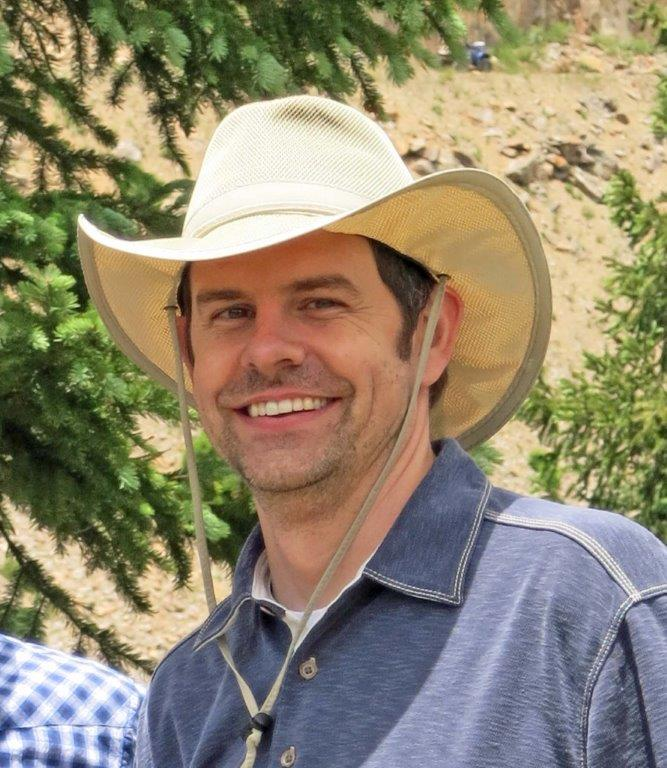
\includegraphics[width=\linewidth]{joemcjoe.jpg}
  \caption{This is Joe.}
  \label{fig:marginfig}
\end{marginfigure}

\section{Proof of Consultation}
Here we provide proof of the consultation.  For example, before meeting I emailed the client to explain the IA project.  We agreed to meet for two hours on Sunday May 3rd at 2:00 PM at the Coffee Lab in Tarrytown.

Include copy of email.  Include a link to his facebook?  Take a picture of him?  Take a picture of your notes from the meeting.

Synopsis of meeting.

\section{Product Rationale}
Describe briefly how to address client needs with solution.  For example, design a Java application that allows student to search a database of colleges according to different criteria.
\cite{Tufte1990}

\section{Background Research}
Required input, calculations, and mathematical models stated in general terms. Although you will be the primary user of the program, input/output should be described for a hypothetical end user who could potentially duplicate or extend your work.\\
References used for background research--minimum of 5. Note that while the Wikipedia is a great place to start, it is not itself a valid reference. Most of these should be from technical journals. Web pages, if appropriate should, at a minimum, include the URL, the author or organization providing the information, and the date. any commonly used form for references is acceptable as long as it contains enough information to find the data.\\
In addition each student should find a research mentor with in-depth expertise of the subject, other than the teacher who is at minimum available by e-mail.
\cite{Tufte1990}
\cite{Tufte2006}
\cite{pkg-geometry}
\cite{Mittelbach2004}
\cite{Bringhurst2005}
\newpage 

\section{Success Criteria}
Must have at minimum an introduction clearly stating the objectives/goals of the solution to the problem and contain an outline, bullet list, or table with the minimum performance and usability criterion so that they are easily scanned.\\

In simulations performance and usability criterion are often defined by simplifying assumptions. For example, in a projectile motion simulation if air resistance is assumed to be negligible, the simulations solutions will only be valid for low speeds.\\

Here make a list with description of each criteria for success of product.
For example:
\begin{description}
\item[\textbf{Existing Database}]  This software should have a database of colleges for the student to look at.  The database should be searchable.
\item[\textbf{Search by Tuition}] Database should be searchable by tuition costs
\item[\textbf{Search by Location}] Database should be searchable by location
\item[\textbf{Search by Majors}] Database should be searchable by available majors
\item[\textbf{Search by Class Size}] Database should be searchable by average class size
\item[\textbf{Saving of Searches}]  Searches can be saved by software
\item[\textbf{Intelligence}] Want student to be able to indicate colleges that are desirable and have software suggest similar colleges.
\item[\textbf{Ordered List}] The returned list of search orders the colleges from best to worst according to criteria of search.
\end{description}

\chapter{Solution Overview}




\section{Record of Tasks}
Here we include a record of tasks.


\begin{fullwidth}


  \begin{center}
  \footnotesize
  \fontfamily{ppl}\selectfont
  \begin{tabular}{lllllc}
    \toprule
    Start Date & Action & Detail & Comments & End Date  & Criterion \\
    \midrule 
    10-10-2010 & \pbox{3cm}{Research college application process} & \pbox{3cm}{I Googled and googled and googled and googled} & \pbox{3cm}{Google is the best thing that has ever happened in the history of googling} & 10-20-2010 & A  \\ \ \\
    10-12-2010 & \pbox{3cm}{Downloading and compiling information for database} & \pbox{3cm}{Went to US World and News Report and downloaded full database using a Python script} & \pbox{3cm}{This process is challenging to do by hand so using the bot was super duper helpful.  Thanks mom.} & 10-22-2010 & B  \\ \ \\
    10-12-2010 & \pbox{3cm}{Project repository initialized} & \pbox{3cm}{Setup a project repository on github titled javabeg under account Tris} & \pbox{3cm}{https://github.com/ Tris/javabeg.git } & 10-22-2010 & B  \\ \ \\
    10-12-2010 & \pbox{3cm}{Developing Classy class} & \pbox{3cm}{Wrote class called Classy with fields x, y, z and methods methodA and methodB} & \pbox{3cm}{These methods allow me to do this and that.  Commit hash: a17ab60957 } & 10-22-2010 & B  \\
    
    \bottomrule
  \end{tabular}
  \end{center}
  \end{fullwidth}

\section{Design Overview}

This section starts by describing an initial design for some of the main objectives that were determined to be the criteria for success. It should consist of the following:
\begin{itemize}
\item a brief verbal description.
\item a block diagram of the program with at least one block describing user input, one describing the manipulation of the input, one describing file I/O, and a 4th describing the output. Bullet statements can be used for the descriptions within each box.
\item The prototype is based on functional decomposition. It is a top-down design that includes NO, repeat NO code. It must include:
\item A brief written summary of the way the program will function that references items 2-4 below. Can be in outline form.
\item Fully annotated computer-generated drawings of the user interface and output. There should be multiple drawings showing the expected output under various conditions.
\item A list identifying all I/O.
\item User feedback in support of the design.. (At least part of this feedback must come from the teacher.)
\end{itemize}

Detail what resources must be collected to execute the project.  If a developer's licence is needed state that.  If any hardware must be obtained state what is needed.  If certain data sets need to be acquired state that.\\ \ \\

The design overview should include an outline test plan.  \\
For example:
State language\\
Explain database structure: College object\\
Search object\\
\\ \ \\
Create a dummy student\\
Create a example college database\\
Test example search with a dummy search
\chapter{Development}
\section{Techniques}
IB asks for the use of techniques which demonstrate a high level of complexity and ingenuity in addressing the scenario identified in criterion A. They are characterized by the appropriate use of existing tools and the techniques are adequate for the task. Their use is explained. All sources are identified.\\
Here we detail techniques used in the project.  Techniques may include the following.

\small
\begin{itemize}
\item Arrays
\item User-defined objects
\item Objects as data records
\item Simple selection (if/else)
\item Complex selection (nested if, if with multiple conditions or switch)
\item Loops (while for)
\item Nested loops
\item User-defined methods
\item User-defined methods with parameters (the parameters have to be useful and used within the method body)
\item User-defined methods with appropriate return values (primitives or objects)
\item Sorting
\item Searching
\item File i/o
\item Use of additional libraries (such as utilities and graphical libraries not included in appendix Java Examination Tool Subsets)
\item Recursion
\item Merging two or more sorted data structures
\item Polymorphism
\item Inheritance
\item Encapsulation
\item Parsing a text file or other data stream
\item Abstract data types
\item Interfaces
\end{itemize}


\chapter{Functionality \& Extensibility}
This section assesses the extent to which the product functions.  A video is used to evidence functionality.  Future modification and expansion is also discussed as detailed in the design and development documentation.

\section{Video}
The video can be found at http://youtube.com/5Tygy

\chapter{Evaluation}

This section must evaluate the effectiveness of the product based on feedback from the client/adviser. This must include direct references to the success criteria identified in criterion A.
The student must recommend proposals for the future improvement of the product.

\section{Client Feedback}
The client feedback should be detailed here.

\section{Success Criteria Review}
Here you go through and repeat the Success criteria list and review the success of each criteria.
\begin{description}
\item[\textbf{Existing Database}]  The database was successfully constructed and includes over 500 colleges and universities in the US.
\item[\textbf{Search by Tuition}] Tution costs were found for each college and included in the database
\item[\textbf{Search by Location}] Location of each school was included by address and GPS coordinates
\item[\textbf{Search by Majors}] Majors were included for colleges with majors.  Schools without majors were still included in the database.
\item[\textbf{Search by Class Size}] Average class size was included in the database
\item[\textbf{Saving of Searches}]  Each user can save five searches 
\item[\textbf{Intelligence}] This feature had limited success
\item[\textbf{Ordered List}] The output of the search gave a match score to each college and listed the colleges in descending order
\end{description}
\cite{Tufte2001}

\section{Future Improvement}
Here you detail future improvement of the project.
\cite{Tufte2006}

\backmatter

\bibliography{sample-handout}
\bibliographystyle{plainnat}


\printindex

\end{document}

